\documentclass[11pt]{article}
\usepackage[top=1in, bottom=1in, left=1in, right=1in]{geometry}

\usepackage{amsmath}
\usepackage{amssymb}
\usepackage{graphicx}

\title{Homework \#12, Due: 4/24 \\Math 181 (Discrete Structures), Spring 2024}
\date{}

\begin{document}

\maketitle

\thispagestyle{empty}

\vspace{-1cm}

Problem 1 is worth 6 points, Problem 2 is worth 2 points, and Problem 3 is worth 2 points, for a total of 10 points. Remember to \emph{show your work} and \emph{explain your answers} on all problems!

\begin{enumerate}

\item Recall that in class we proved the Binomial Theorem: $(x+y)^n = \sum_{k=0}^{n} C(n,k) x^{k} y^{n-k}$. Use the binomial theorem to prove the following identities for the binomial coefficients $C(n,k)$:
\begin{enumerate}
\item $\sum_{k=0}^{n} 2^k \cdot C(n,k) = 3^n$
\item $\sum_{k=0}^{n} (-1)^{n-k} \cdot 2^k \cdot C(n,k) = 1$
\item $\sum_{k=0}^{n} k \cdot C(n,k) = n \cdot 2^{n-1}$ \\[5pt] \qquad {\bf Hint:} take the \emph{derivative}, with respect to $x$, of the binomial theorem identity.
\end{enumerate}

\item We saw how the $C(n,k)$ form Pascal's Triangle. Here are the first 16 rows of Pascal's Triangle:
\begin{center}
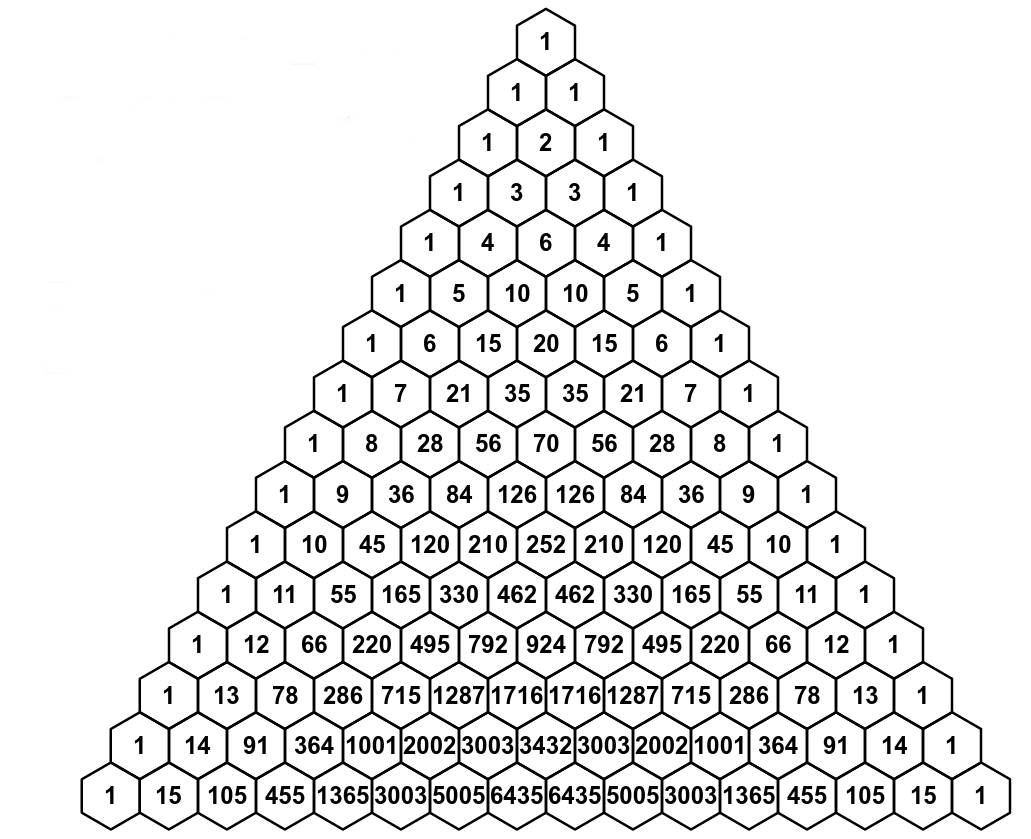
\includegraphics[width=4in]{pascal.png}
\end{center}
Fill in all of the odd values in the above triangle, and leave the even values unfilled. Describe the resulting pattern that you see.

\item Show that any subset of $X = \{1,2,3,4,5,6\}$ of size at least $4$ contains a pair of elements whose sum is $7$. {\bf Hint}: use the Pigeonhole Principle, where the ``holes'' are the pairs of numbers in~$X$ summing to $7$.

\end{enumerate}

\end{document}
